% !TEX root = ../thesis.tex
% !TEX spellcheck = en-US

%% Leave first page empty
\thispagestyle{empty}

\section{Introduction}

Language is one of the most complex behaviors our species has developed. We humans use it to efficiently transport knowledge between individuals and communicate even the most abstract concepts with it. It takes children years to learn to learn express their thoughts and the subtle nuances of one's language give a glimpse one's cultural environment and upbringing, one's emotional state and one's intellect.

Not surprisingly in the field of \gls{AI} and especially \gls{ML} building computer systems with linguistic capabilities and solving language-based problems poses one of the hardest challenges and has motivated decades of research in Computational Linguistics. In fact many of the famous test for universal machine intelligence are based on linguistic capabilities, among them the famous \emph{Turing test} by~\cite{Turing:1950aa} where the task is for a human judge to determine whether he is having a conversation with a human or a machine in order to determine if the machine can be called intelligent, or the \emph{compression test} proposed by~\cite{Mahoney:1999aa}, where a human's and machine's capability to predict missing words given a context is tested.

This thesis explores the specific task of predicting the semantic structure of job advertisements as a specific example of such a language-based task that turns out to be difficult even for humans to do.

The work was done in close collaboration with the Helsinki-based media and learning company \emph{Sanoma}\footnote{\textquote{Sanoma is a front running consumer media and learning company in Europe. In Finland and the Netherlands we are the market leading media company with a broad presence across multiple platforms. In Belgium we are among the Top 5. Our main markets in learning are Belgium, Finland, the Netherlands, Poland and Sweden. We entertain, inform, educate and inspire millions of people every day. We employ some 7,500 professional employees operating in Europe.}, Source: \url{http://www.sanoma.com/en/who-we-are}, visited 06.06.2016} and the research motivation was thus constantly tied back into real world challenges in the scope of Sanoma's business needs.

\subsection{Problem Statement}

The problem addressed during with this thesis to better understand the structure of job advertisements. In particular job postings typically consist of several parts with a certain function or theme: Usually the company is introduced, the job is described with it's tasks and responsibilities, the requirements for the job are listed, then benefits and offerings by the company are named and the reader is asked to apply in a specified way he or she is interested.
Almost all of the text of a job description falls into these categories\footnote{Only about 4\% of the sentences collected for evaluating the final experiments in this thesis were sorted into the category \emph{other} while the rest falls into either of the categories described. This is described in more detail in Section~\ref{subs:Multi-class Sentence Classification}} and the task can thus be posed as predicting a category for each sentence in a job advertisement, that corresponds with this sentence belonging to one of the job ads' parts as described above.
This is a challenging problem in itself but can further be used to extract certain functional parts of each job ad, to study a possible correlation between structural patterns and the reach and success of an ad and so forth. The problem therefore can be labelled as \emph{Text Categorization} or \emph{Text Classification} as referred to in the scientific literature.


\subsection{Need Statement and Motivation}

% -- need statement

Today's media and education, the basis of Sanoma's core businesses, are undergoing drastic and fundamental transformations that are currently disrupting whole industries. Usage of digital media as a source of information has long surpassed print media. Sanoma's most well-known product, Finland's biggest daily newspaper \emph{Helsingin Sanomat}, lost 6\% of its circulation only in 2015\footnote{Source: http://www.digitalnewsreport.org/survey/2016/finland-2016/, visited 27.07.2016}, while the wide-spread use of social media challenges traditional ways we access information. Similarly in the field of education, with the rise of Massive open online course (MOOCs), traditional learning settings are challenged and the need for advanced techniques for data processing and analysis increases, e.g.\ to personalize and adapt the learning experience to each individual user and at the same time identify trends across large groups of learners to better meet the needs of education.

Sanoma provides a recruitment platform named \emph{Oikotie Työpaikat}. The service is in direct competition several other international players in the recruitment industry. Through this and other services Sanoma's collects large amounts of user-generated data, offering the potential to be leveraged for machine learning solutions to provide value for their users and innovate and enrich the company's offerings.
This was the company's initial motivation for this thesis project --- To explore ways to leverage user-generated data to potentially.

% -- research motivation

% -- personal motivation

From a personal perspective this work was interesting as offered many research possibilities while at the same time being relevant for and inspired by real life applications. The complex nature of \acrlong{CL} with its proximity to the general study of machine intelligence and the high interpretability of problems makes poses makes it a fascinating problem domain. This presented a great challenge to learn balancing scientific research objectives and yet exploring potential business and user needs, learn on new fronts and deepen the knowledge in others and apply it to real data.

\subsection{Related work}
\label{sub:Related work}

The problem of \gls{TC}, also known as Text Categorization, is one of the various challenges in the thriving fields of \acrfull{CL} and \gls{NLP}. These areas of research have started out as theoretically challenging but rather marginally popular fields between \acrfull{AI} and formal linguistics and have since exploded in terms of interest with their applications being deployed currently at large scale to practically all kinds of consumer products such as smart phones and home entertainment systems as well as digital services like social networks, automatic translation engines and conversational agents.
Today there are textbooks dedicated specifically to this area, such as~\cite{Manning:1999aa},~\cite{Jurafsky:2014aa} and~\cite{Clark:2013aa} There is also much overlap to the field of \gls{IR} that rose to popularity during the late 1980's due to the Internet starting to become a mainstream medium (see~\cite{Manning:2008aa},~\cite{Leskovec:2014aa} and the classic work by~\cite{Rijsbergen:1979aa}).

\subsubsection*{Syntactics, Semantics, and Pragmatics}
\label{subs:Vogues in NLP: Syntactics, Semantics, and Pragmatics}

The field of Natural Language Processing has undergone different trends of modeling approaches to tackle its challenges.~\cite{Cambria:2014aa} identify these as three main trend curves focusing on \emph{Syntactics}, \emph{Semantics}, and \emph{Pragmatics}. According to the authors the first trend of syntax-centered NLP is still prevalent and is based on algorithms that more or less directly operate on the words found in the processed texts.
The second trend operates on the semantics of text, thus being able to potentially tackle more challenging problems by addressing increasingly subtle notions of meaning and context. According to the author these types of approaches are still in the early phase but at the verge of being adapted by a broader audience of researchers and practitioners in the field.
The last trend curve of pragmatics regards the yet more complex issue of modeling inherent narratives in language where so far only pioneering work has been done but which, according to the authors, will lead to tackling problems of natural language understanding.

\subsubsection*{The Text Classification Problem}
\label{subs:The Text Classification Problem}

The problem of \acrfull{TC} specifically has seen many evolving fashions of approaches and more or less loosely follows the three trend curves described above. \gls{TC} has been of immense interest for several decades now due to the exponentially increasing amounts of text data being recorded in forms of e.g.\ user generated content through social networks and through the increased digitalization of our daily lives. Its applications reach from document filtering, automated metadata generation such as language classification to automatic email labeling, spam identification and sentiment detection, amongst others.

\acrlong{TC} is nowadays covered in standard works of \acrlong{IR} and \acrlong{ML}, such as~\cite{Manning:2008aa}. As~\cite{Sebastiani:2002aa} points out it is important to mention that the term \emph{automatic text classification} has also been used referring to different problems: \textquote{Aside from (i) the automatic assignment of documents to a predefined set of categories [\ldots], the term has also been used to mean (ii) the automatic identification of such a set of categories (e.g.,~\cite{Borko:1963aa}), or (iii) the automatic identification of such a set of categories and the grouping of documents under them (e.g.,~\cite{Merkl:1998aa}), a task usually called text clustering, or (iv) any activity of placing text items into groups, a task that has thus both TC and text clustering as particular instances~\cite{Manning:1999aa}}

\subsubsection*{Early Work and Syntactic Approaches}
\label{subs:Early Work and Syntactic Approaches}

Early approaches towards solving \acrlong{TC} tasks in the 1980's were in often based on expert systems consisting of sets of manually created logical rules, deciding upon the category of a text segment if a certain formula applies. As discussed by~\cite{Sebastiani:2002aa} the biggest downside is known as the \emph{knowledge acquisition bottleneck} which refers to the fact that each rule has to be manually created. In the 1980's machine \acrfull{ML} became more common where a \emph{classifier} automatically learns the attributes of the data and its association with the given data labels using a model that allows to then infer the categories for unseen data. This setting is called \gls{Supervised Learning} as labels for the data are given and predicted.

\acrshort{ML} approaches have since been developed in countless variations. As described earlier syntax-based approaches are still very common and most follow a classic pipeline of \emph{feature extraction} or \emph{indexing} of documents followed by \emph{inductive construction} of a classifier that is lastly evaluated by a measure of effectiveness. A very successful approach to feature extraction has been the introduction of N-Gram based models, also called \emph{bag-of-words} models, which that are based on word-cooccurrence frequencies of the terms that are present in the data (see Section~\ref{subs:N-gram Models (Methods)} for an introduction).
As~\cite{Mikolov:2012aa} explains \textquote{the most significant advantages of models based on n-gram statistics are speed (probabilities of n-grams are stored in precomputed tables), reliability coming from simplicity, and generality (models can be applied to any domain or language effortlessly, as long as there exists some training data). N-gram models are today still considered as state of the art not because there are no better techniques, but because those better techniques are computationally much more complex, and provide just marginal improvements, not critical for success of given application.}
The limitation of such models is that their statistics are directly based on word co-occurrences and thus exponentially increase in size as the desired context to be captured is expanded, making them infeasible to adapt to longer text sequences.

\subsubsection*{Semantic Approaches and Representation Learning}
\label{subs:Semantic Approaches and Representation Learning}

Recently approaches from the field of \emph{Representation Learning}, have found their way into and gained tremendous traction in the \gls{NLP} research community. Traditional techniques such as N-gram models, now also referred to as \gls{Feature Engineering} approaches, use prior domain or expert knowledge in order to build data representations that are effective in combination with a classifier. But as~\cite{Bengio:2013aa} point out this is a laborious and time-consuming task that only exposes the weakness from a Machine Learning point of view by not automatically learning such representations --- a challenge representation learning aims to address. Beyond that, with regards to \gls{CL} problems, most \gls{Feature Engineering} techniques do not capture well the semantics of language.

One example particularly popular method called \emph{word2vec} was introduced by \cite{Mikolov:2013ad} and learns word representation vectors, so-called \emph{word embeddings}, through a context-prediction task. This produces extremely rich representations capturing many subtleties in the layers of meaning of words\cite{Mikolov:2013ab}. Another approach related to \gls{Representation Learning} under the name of Transfer Learning has been proposed by~\cite{Do:2006aa}. Similarly, in attempts to find more expressive ways of modeling semantics of language several breakthrough achievements in \acrshort{NLP} have been made using various \gls{Deep Learning} based methods --- a related trend that the field has picked up.
\cite{Collobert:2011aa} succesfully applied a \acrfull{CNN} architecture to a number of standard problems in \gls{NLP} with the intention of minimizing the domain knowledge introduced: \textquote{The design of this system was determined by our desire to avoid task-specific engineering as much as possible. Instead we rely on very large unlabeled datasets and let the training algorithm discover internal representations that prove useful for all the tasks of interest.}.
Later~\cite{Kim:2014aa} improved the method slightly, improving on state-of-the-art results in 4 out of 7 of these standard problems. Numerous related work was done building on similar ideas, such as using a \acrshort{CNN} on character level resolution for \gls{TC}~\cite{Zhang:2015aa}, Multitask Learning and Semi-Supervised Learning to improve the generalization of the shared tasks\cite{Collobert:2008aa} and using \glspl{RNN}~\cite{Liu:2016aa}. Just recently facebook research released a tool called \emph{fastText}\footnote{The tool is publicly available on \gls{GitHub}: \url{https://github.com/facebookresearch/fastText}} for \gls{TC} with a focus fast run-time while still achieving close to state-of-the-art results. The related publications draw heavily on previous work on word embeddings and similar techniques (see~\cite{Joulin:2016aa} and~\cite{Bojanowski:2016aa}).

\subsubsection*{Further Related Work and Focus of This Thesis}
\label{subs:Further Related Work and Focus of This Thesis}

Numerous other classes of approaches exist and have been explored with varying popularity such as \gls{TC} using String Kernels~\cite{Lodhi:2002aa}, \gls{EM} (\cite{Nigam:2000aa} and~\cite{McCallum:1999aa}), \gls{SOM}~\cite{Merkl:1998aa} and using a \gls{CRF} for sequence labeing~\cite{Lafferty:2001aa}.
Also problem areas from the field of \gls{Unsupervised Learning} are related with techniques such as~\gls{LDA} \cite{Blei:2003aa} for \gls{Topic Modeling} where labels for text documents are found without providing a \gls{Ground Truth} beforehand. However this work specifically focuses on comparing traditional syntactic approaches to more recent semantic ones, focusing on ideas from \gls{Representation Learning} and \gls{Deep Learning}, in particular \glspl{RNN}.

\subsection{Research Scope and Objectives}
\label{sub:Research Scope and Objectives}

This thesis was initiated as a research project for Sanoma's recruitment platform \gls{Oikotie Tyopaikat} with the intention of exploring interesting and novel ways to use the various data generated through the use of this service. The research objectives were stated as follows:

\blockquote{Find an application of data mining / machine learning to the customer-generated data on the recruitment platform Oikotie Työpaikat which has the potential of bringing value to the user of the platform and is technically feasible in the scope of a master’s thesis. Further define and investigate a research problem that is essential to this application by researching literature and previous work on similar problems trying different approaches based on the literature using the results and learnings to create an improved approach.}

In order to meet these objectives a predefined development process was applied that will be explained in the next section.

\subsection{Methodological Approach}
\label{sub:Methodological Approach}

\begin{figure}[h]
    \centering
    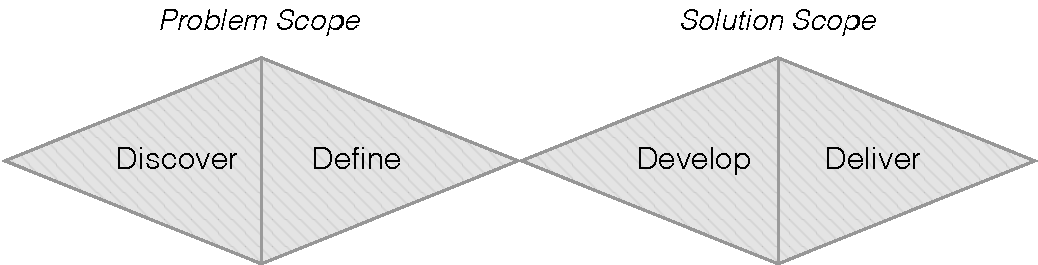
\includegraphics[width=\textwidth]{img/double-diamond.pdf}
    \caption{Design process for this thesis, adapted from the \emph{Double Diamond Process} developed by the British Design Council (see~\cite{Council:2007aa})}
\label{fig:double-diamond}
\end{figure}

The development process for this thesis project was adapted from the Double Diamond design process developed by the by the British Design Council in 2005 (see ~\cite{Council:2007aa}). A design process is \textquote{the specific series of events, actions or methods by which a procedure or set of procedures are followed, in order to achieve an intended purpose, goal or outcome.}~\cite{Best:2006aa}.
The Double Diamond process consists of iterative, explorative learning phases where first a problem worth solving is found within the \emph{Problem Scope} and afterwards the best solution is formed in the \emph{Solution Scope}. Both scopes are navigated through a so-called divergence phase where the space explored for finding possibilities followed by a convergence phase where the options are reduced and combined. These phases, as illustrated in Figure~\ref{fig:double-diamond}, are called \emph{Discovery Phase} and \emph{Definition Phase} in the Problem Scope and \emph{Development Phase} and \emph{Delivery Phase} in the Solution Scope and briefly described next:

\paragraph{Discovery Phase}
\label{par:Discovery Phase}
In the Discovery Phase opportunities for problems worth solving are evaluated. Often their potential is measured in terms of economic impact (financial viability), attractiveness to and impact on users (desirability) and the level of technological challenge (feasibility).
These aspects require different ways of testing and as the priority in this work lays on primarily on evaluating the technical challenge the main tools were prototyping, technical benchmarking and literature research.

\paragraph{Definition Phase}
\label{par:Definition Phase}
The aim of the Definition Phase is to compile the learnings from the Discovery Phase and find the problem that has the most potential and will be tackled. This is done by iteratively reframing the problem and testing the implications of this definition.
Thus the final problem definition is often not simply selected but developed through a series of steps of refining the problem, testing and learning.

\paragraph{Development Phase}
\label{par:Development Phase}
When the final problem definition has been set the Development Phase aims to produce a wide variety of potential approaches to solving this problem. Here existing approaches are benchmarked and tested, and combined with new ideas, again through a \emph{test, learn, rescope} cycle.
With regards to this work literature research was combined with testing of various methods and evaluating there performance to learn which approaches work best and how they could be improved, combined or built upon.

\paragraph{Delivery Phase}
\label{par:Delivery Phase}
During the Delivery Phase the best possible solution is chosen through refinement of the different approaches that were evaluated. At the end there stands a result of the whole process, in this case a comprehensive evaluation and conclusion on the approaches.

\subsection{Results}

This thesis shows that recent approaches from Representation Learning and Sequential Modeling techniques are competitive and even yield better performance for text classification than traditional N-Gram based models that are still considered state-of-the art and widely applied. This is confirms the assumption that data-driven approaches are a promising direction for \acrfull{CL} and \acrfull{NLP} and beyond as they are more informed by the actual structure in the data than by model decisions of the algorithm designer using knowledge about the problem domain. Further sequential modeling of text on a character level is shown to yield competitive results while being even more domain-agnostic as the only knowledge provided is the difference between characters.
